\documentclass[%
 reprint,
%superscriptaddress,
%groupedaddress,
%unsortedaddress,
%runinaddress,
%frontmatterverbose, 
%preprint,
%showpacs,preprintnumbers,
%nofootinbib,
%nobibnotes,
%bibnotes,
 amsmath,amssymb,
 aps,
%pra,
%prb,
%rmp,
%prstab,
%prstper,
%floatfix,
]{revtex4-1}
\usepackage{gensymb}
\usepackage{listings}
\usepackage{graphicx}% Include figure files
\usepackage{dcolumn}% Align table columns on decimal point
\usepackage{bm}% bold math
%\usepackage{hyperref}% add hypertext capabilities
%\usepackage[mathlines]{lineno}% Enable numbering of text and display math
%\linenumbers\relax % Commence numbering lines

%\usepackage[showframe,%Uncomment any one of the following lines to test 
%%scale=0.7, marginratio={1:1, 2:3}, ignoreall,% default settings
%%text={7in,10in},centering,
%%margin=1.5in,
%%total={6.5in,8.75in}, top=1.2in, left=0.9in, includefoot,
%%height=10in,a5paper,hmargin={3cm,0.8in},
%]{geometry}
\usepackage[margin=25mm]{geometry}
%\usepackage{booktabs}
\usepackage{changepage}
\usepackage{mathcomp}
\usepackage[english]{babel}
\usepackage{siunitx}
\DeclareSIUnit\minute{min}
\usepackage{amsmath,mathrsfs,amsfonts,amssymb,amsthm } %permette di mettere formule una sotto l'altra,
%dovrebbe scrivere lettere corsive eleganti con "\mathscr{--},"
% permette di definire insiemi numerici con \mathbb{""},
\usepackage[utf8]{inputenc} %accenti
\theoremstyle{plain} 
\theoremstyle{definition}
\newtheorem{defn}{Def}[section]
\theoremstyle{plain}
\newtheorem{thm}{Theorem}[section] 
\newcommand{\R}{\mathbb{R}}
\newcommand{\N}{\mathbb{N}}
\newcommand{\off}{\text{off}}
\newcommand{\mat}{\text{Mat}}
\newcommand{\B}{\mathbf{B}}
\newcommand{\A}{\mathbf{A}}
%\newcommand{\S}{\mathbf{S}}
\newcommand{\open}{\left}
\newcommand{\close}{\right}
\newcommand{\void}{\varnothing}
\newcommand{\xslash}{\setminus}
\usepackage{tikz}
%\newcommand{\fnorm}{\lVert #1 \rVert_F}
\newcommand{\tikzcircle}[2][red,fill=red]{\tikz[baseline=-0.5ex]\draw[#1,radius=#2] (0,0) circle ;}

\usepackage[T1]{fontenc}
\usepackage{subfig}
\usepackage{caption}
\usepackage{subfig}
\usepackage{booktabs}
\usepackage{float}
\usepackage{mathdots}
\usepackage{mathrsfs}
\usepackage{braket}
\usepackage{hyperref}
\usepackage{float}

\usepackage{pgfplots}
\usepackage{circuitikz}
\usepackage{hyperref}
\usepackage{tkz-tab}
\usepackage{caption}
\usetikzlibrary{backgrounds,automata}
\pgfplotsset{/pgf/number format/use comma,compat=newest}
\usetikzlibrary{graphs,shapes,positioning,shadows}

\usepackage{colortbl}
\newcommand{\blue}[1]{\textcolor{blue}{#1}}
\newcommand{\red}[1]{\textcolor{red}{#1}}
\newcommand{\green}[1]{\textcolor{green}{#1}}
\newcommand{\magenta}[1]{\textcolor{magenta}{#1}}
\newcommand{\cyan}[1]{\textcolor{cyan}{#1}}
\newcommand{\yellow}[1]{\textcolor{yellow}{#1}}
\newcommand{\grey}[1]{\textcolor{grey}{#1}}
\newcommand{\abs}[1]{\lvert#1\rvert}
\newcommand{\mean}[1]{\langle #1\rangle}
\DeclareSIUnit\year{yr}
\begin{document}

\preprint{APS/123-QED}

\title{FYS 3150 - Project 4}% Force line breaks with \\
%\thanks{A footnote to the article title}%

\author{Federico Nardi}
% \altaffiliation[Also at ]{Physics Department, XYZ University.}%Lines break automatically or can be forced with \\
%\author{}%
% \email{Second.Author@institution.edu}
\affiliation{University of Oslo, Department of Physics}
% Authors' institution and/or address\\
% This line break forced with \textbackslash\textbackslash
%}%

%\collaboration{MUSO Collaboration}%\noaffiliation

\date{\today}% It is always \today, today,
             %  but any date may be explicitly specified

\begin{abstract}
\textbf{In this project we use a Monte Carlo approach based on Metropolis algorithm to simulate a 2D binary lattice with Ising model for magnetic interactions and study it by analizing its expectation values. We first set a small lattice and compare the numerical values with the analytical ones to see when we have a good agreement. Then we increase the lattice size and study the evolution of the system towards equilibrium; we also study the energy distribution of the energies referring it to Boltzmann distribution. Eventually we simulate bigger lattices (40x40,60x60,80x80,100x100) and study the temperature-dependence of the expectation values. We manage to characterize a second-order phase transition and to get the values ot critical temperature for each lattice size. We also extend our result to an infinite 2D lattice and get for it a value of critical temperature $(T_c(L=\infty) = (2.261\pm0.008)Jk_B^{-1})$ that is compatible with the exact analytical one.}
%\centering{Abstract}

%\begin{description}
%\item[Usage]
%Secondary publications and information retrieval purposes.
%\item[PACS numbers]
%May be entered using the \verb+\pacs{#1}+ command.
%\item[Structure]
%You may use the \texttt{description} environment to structure your abstract;
%use the optional argument of the \verb+\item+ command to give the category of each item. 
%\end{description}

\begin{itemize}
\item URL to GitHub folder of the code: \url{https://github.com/FedericoNardi/Computational/Project 4}
\end{itemize}
\end{abstract}

\pacs{Valid PACS appear here}% PACS, the Physics and Astronomy
                             % Classification Scheme.
%\keywords{Suggested keywords}%Use showkeys class option if keyword
                              %display desired
\maketitle

%\tableofcontents
\section{Introduction}
The aim of this project is to simulate a 2D binary lattice with Ising model for magnetic interactions and extend our results to an infinite 2D lattice. To do this we will use a Monte Carlo (MC) approach based on Metropolis algorithm.
At first we set a $2\times2$ lattice and analyze the efficiency of our algorithm by determining the number of MC cycles needed to get a good agreement between numerical and theoretical values. Then we increase the size of our lattice to $20\times20$ and study thermodinamically the evolution of our system towards equilibrium, starting by both an ordered and random configuration. We also analyze the energy distribution of the states and comment its behaviour referring to Boltzmann distribution. 
We eventually increase further the size of the lattice and study the behaviour of expectation values close to a phase transition. We manage to find a critical temperature for each lattice size and extend our result for a infinite 2D lattice.


\section{Methods and algorithms}
	\subsection{The Ising model}
	We are considering a 2D magnetic system represented by a binary $N\times N$ spin lattice where the possible values are $s=1,\, s=-1$. We compute the total magnetization  for a configuration (microstate) by summing over the spin moments: 
	\begin{align*}
		M_i=\sum_{k,l=1}^{N}s_{kl}.
	\end{align*} 
	The energy of this system $i$ is given by summing over the neighbour pairs only:
	\begin{align*}
		E_i = -J\sum_{<k,l>=1}^{N}s_ks_l
	\end{align*}
	where the coupling term $J$ expresses the interaction between two neighbouring spins.
	Since we ideally want to relate our results to an infinite lattice, we choose to use \textit{periodic boundary conditions} when computing the total energy of the system: when we consider a spin at the end of a row $s_{j,N}$ or a column $s_{N,k}$, it will interact with its neigbour $N+1$ that will assume the value -respectively- $s_{j,1}$ and $s_{1,k}$.
	Thermodynamically, our system is a \textit{canonical ensemble} and the energy distribution of the microstates $E_i$ follows the Boltzmann distribution:
	\begin{align*}
		p(E_i) = \frac{e^{-\beta E_i}}{Z}
	\end{align*}
	where $\beta=(k_BT)^{-1}$ is the Boltzmann factor given by the inverse product between Boltzmann constant $k_B$ and absolute temperature T. Z is the normalization constant given by the partition function, summing over all the microstates $i$:
	\begin{align*}
		Z=\sum_{i}e^{-\beta E_i}
	\end{align*}
	
	We can thus compute some expectation values such as
	
	\paragraph*{\textbf{Mean Energy}}
	\begin{align*}
	\begin{split}
		\mean{E}&=K_BT^2(\partial_T\ln Z)_{N,V}\\
		&=\frac{1}{Z}\sum_i E_ie^{-\beta E_i}
	\end{split}
	\end{align*}
	We can get the specific heat at constant volume $c_V$ by computing its variance $\sigma_E^2=\mean{E^2} - \mean{E}^2$:
	\begin{align*}
	c_V=\frac{1}{k_BT^2}\sigma_E^2
	\end{align*}
	
	\paragraph*{\textbf{Mean magnetization}}
	\begin{align*}
	\begin{split}
	\mean{M}=\frac{1}{Z}\sum_i M_ie^{-\beta E_i}
	\end{split}
	\end{align*}
	Its variance $\mean{M^2}-\mean{M}^2$ allows us to define the susceptibility $\chi$:
	\begin{align*}
	\chi=\frac{1}{k_BT}\sigma_M^2
	\end{align*}
	
	For example, in a $2\times 2$ lattice, there are 3 different macrostates for energy $(-8J,0,8J)$ and 5 for magnetization $(-4,-2,0,2,4)$ \cite{compnotes} we can get the values:
	\begin{align}
		\label{EValsModel}
		\begin{split}
		&Z = 4\big(3 + \cosh(8J\beta)\big)\\
		&\mean{E} = -8J\frac{\sinh(8J\beta)}{3 + \cosh(8J\beta)}\\
		&\mean{E^2} = 32J^2\frac{\cosh(8J\beta)}{3 + \cosh(8J\beta)}\\
		&c_V= \frac{32J^2}{k_BT^2}\bigg( \frac{\cosh(8J\beta)}{3 + \cosh(8J\beta)} - \frac{\sinh^2(8J\beta)}{(3 + \cosh(8J\beta))^2}\bigg)\\
		&\mean{M} = 0\\
		&\mean{M^2} = 8\frac{e^{8J\beta}+1}{3 + \cosh(8J\beta)} \\
		&\chi = \frac{8}{k_BT}\frac{e^{8J\beta}+1}{3 + \cosh(8J\beta)}
		\end{split}
	\end{align}

	The potential that determines the evolution of the system towards equilibrium is \textit{Helmoltz' free energy}, defined as:
	\begin{align*}
	\Phi = -k_BT\ln Z = \mean{E} - TS
	\end{align*}
	where $S$ is the entropy of the system.
	It expresses the balance two leading driving forces of classical physics such as the tendency to the minimum energy state and the highest entropy state; this means that the equilibrium state of our system ($\Delta\Phi=0$) may not correspond to the minimum energy state because of entropy, that drives it towards disorder.\\
	
	Our final aim is to study the behaviour of the system depending on the lattice size tor temperatures close to a critical temperature $T_c$. In this regime we can analyze a phase transition, that could be of the first order -with discontinuity in the mean energy $\mean{E}$- or upper (essentially depending on which order of Helmholtz' free energy derivative we have a divergency). In our case we expect a second-order transition, where the values close to $T_c$ obey a power law such as $|T_c-T|^{k}$:
	\begin{align*}
	\begin{split}
		&\mean{M(T)}\sim(T-T_c)^\beta\\
		&c_V(T)\sim|T_c-T|^{-\alpha}\\
		&\chi(T)\sim|T_c-T|^{-\gamma}\\
		&\text{with }\beta=\frac{1}{8},\quad\alpha=0,\quad\gamma=\frac{7}{4}.
	\end{split}
	\end{align*}
	 For such a system we can define a correlation length $\xi\sim|T_c-T|^\nu$ that is expected to become bigger as the system approaches to $T_c$ (the spins will become more and more correlated). 
	 It is also possible to relate the behaviour at finite lattices tho the infinite one:
	 \begin{align}
		 \label{critictemp}
		 T_c(L) = T_c(L=\infty) + aL^{-\frac{1}{\nu}}
	 \end{align} 
	 where $a$ is a constant and for our analysis we will use the exact value $\nu=1$. The exact result, found analytically by L. Onsager \cite{compnotes} is:
	 \begin{align}
		 T_c= \frac{2}{\ln(1+\sqrt{2})}\frac{J}{k_B}\simeq 2.269\frac{J}{k_B}
	 \end{align}
	
	\subsection{The Algorithm, Metropolis selection rule}
	The algorithm implemented on the code is quite straightforward and exploits the fact that the time evolution of our system can be considered a Markov chain. 
	After initialising the first variables (lattice dimension, number of Monte Carlo (MC) cycles) and looping over a set of temperatures, the nucleus of the program is in the function $\mathtt{MetropolisSampling}$. Here the function $\mathtt{InitializeLattice}$ fills the lattice matrix with the values of spins, at first setting them all up $(+1)$; later it uses an RNG (Mersenne-Twister) to fill it randomly with $+1$ or $-1$:
	\begin{lstlisting}
 for(int x =0; x < NSpins; x++) {
 for (int y= 0; y < NSpins; y++){
 // Set RNG for lattice
 ...
 // Random choice of spin value
 if(RandomNumberGenerator(gen)<0.5){
 	 SpinMatrix[x][y] = 1.0;
 } else SpinMatrix[x][y] = -1.0;
	\end{lstlisting}
	the function computes also the initial energy (with PBC) and magnetic moment of the system.
	After that the RNG is initialized with the seed and we set a loop over the selected number of Monte Carlo cycles.
	Every cycle consists in looping over all the spins of the lattice and for every loop the flipping of a random spin is proposed; the selection rule for the move comes from Metropolis algorithm that will be shown later. At the end of each MC loop the expectation values are updated and printed on an output file. The printing function $\mathtt{WriteResultstoFile}$ normalizes the expectation values by the number of spins (squared if computing variances) in order to get as output intensive variables, easier to be compared between different lattice-sizes results.
	The final code is parallelized with functions from $\mathtt{MPI}$ library, in order to generate data faster for bigger lattice dimensions: by running the data-generating part of the code in more processors it is possible to get number-of-processors times more data in the same time of running the non-parallelized code. Here the local expectation values are summed and collected in a single array $\mathtt{TotalExpectationValues}$ by the function $\mathtt{MPI\_Reduce}$. The output values are the ones from this array, already normalized by the number of cycles times number of processes.
	Note that we could first flip the spins and then compute the total energy of the system and perform Metropolis algo at the end of each MC cycle. We chose instead to compute the energy and run Metropolis selection after flipping each spin since there are only five possible values of $\Delta E$ that can be precalculated, allowing us to save a large amount of flops. The two methods are mathematically equivalent, but the first is computationally more efficient.\\
	
	\subsubsection*{\textbf{Metropolis algorithm}}
	Metropolis algorithm is based on Markov chains and makes use of ergodic hypothesis and detailed balance.
	We want to compute the probability of a transition in the state $w_i$ after a time $\varepsilon$:
	\begin{align*}
	w_i(t+\varepsilon) = \sum_j W_{j\rightarrow i} w_j(t)
	\end{align*} 
	where $W_{j\rightarrow i}$ is the transition probability from a state $j$ to the state $i$. Since $W_{j\rightarrow i}$ is unknown, we try to model it by splitting it into two probabilities: $\mathscr{T}_{j\rightarrow i}$ -the probability of making a transition- and $\mathscr{A}_{j\rightarrow i}$ -the probability of accepting the move-:
	\begin{align*}
	W(j\rightarrow i)=\mathscr{T}_{j\rightarrow i}\mathscr{A}_{j\rightarrow i}.
	\end{align*}
	Dynamically, the transition to the state $i$ can be obtained by simply moving from a state $j$ to $i$ or, if $i$ was already the current state at $t$, by rejecting any move from it to any another state $j$; thus the transition probability is:
	\begin{align*}
	w_i(t+\varepsilon) = \sum_j\big[ w_j(t)\mathscr{T}_{j\rightarrow i}\mathscr{A}_{j\rightarrow i} + w_i(t)\mathscr{T}_{i\rightarrow j}\big(1-\mathscr{A}_{i\rightarrow j}\big) \big].
	\end{align*}
	Since $\sum_j \mathscr{T}_{i\rightarrow j} = 1$ (normalization condition), we get:
	\begin{align*}
	w_i(t+\varepsilon)-w_i(t)=  \sum_j\big[ w_j(t)\mathscr{T}_{j\rightarrow i}\mathscr{A}_{j\rightarrow i} - w_i(t)\mathscr{T}_{i \rightarrow j}\mathscr{A}_{i \rightarrow j} \big]
	\end{align*}
	At the equilibrium $(t\rightarrow\infty)$ we loose the temporal dependence and we get:
	\begin{align*}
	\sum_j w_j\mathscr{T}_{j\rightarrow i}\mathscr{A}_{j\rightarrow i} = \sum_j w_i\mathscr{T}_{i \rightarrow j}\mathscr{A}_{i \rightarrow j}.
	\end{align*}
	However, since this condition cannot guarantee cyclic solutions and the system may not reach the equilibrium state, we need a stronger relation that comes from \textit{detailed balance} condition:
	\begin{align*}
	w_j\mathscr{T}_{j\rightarrow i}\mathscr{A}_{j\rightarrow i} =  w_i\mathscr{T}_{i \rightarrow j}\mathscr{A}_{i \rightarrow j}.
	\end{align*} 
	In our case, the likelihoods $w_k$ are given by the Boltzmann distribution and $\mathscr{T}_{i \rightarrow j}=\mathscr{T}_{i \rightarrow j}=N_{spins}^{-1}$ is the probability of picking one random spin, given by uniform distribution:
	\begin{align*}
	\frac{\mathscr{A}_{i \rightarrow j}}{\mathscr{A}_{j \rightarrow i}}=e^{-\beta(E_j-E_i)}=e^{-\beta\Delta E}
	\end{align*}
	If $E_i<E_j$, we set $\mathscr{A}_{j \rightarrow i}=1$ to be the largest acceptance value since we are moving to a lower energy state. However, accepting only these kind of moves will lead to biased values as the ergodic hypothesis is violated: for a Markov process it should be possible to reach any possible state from any starting point -if carried on for long enough time-. Hence, we accept the proposed move if the exponential $e^{-\beta\Delta E}$ is bigger than a random number generated in the interval $[0,1]$.
		
\section{Our results}
Note: All the expectation values in our analysis are normalized by the total number of spins in order to get an intensive value.
\subsection{$2\times2$ lattice}
As first, we set a $2\times2$ lattice with $T=1.0\,J/k_B$ and see how many MC cycles we need to perform in order to reach a good compatibility with the values from our model (eq. \ref{EValsModel}). In Figure 1 we see that for more than $5\times10^5$ cycles all the numerical values (except the specific heat) differ from the theoretical ones by less than $\SI{1}{\percent}$ (the values are stated in Table I). 

\begin{table}[h!]
		\label{tab:evals}
		\caption{In the table are displayed the numerical expectation values for five numbers of MC cycles as well as the theoretical ones computed from the model.}
\begin{tabular}{ccccc}
		\toprule
		cycles & $\mean{E}$ & $c_V$ & $|M|$ & $\chi$ \\
		\midrule
		$10^4$ & $-1.9968$ & $0.0246$ & $0.0988$ & $3.9289$ \\
		$10^5$ & $-1.9957$ & $0.0345$ & $0.0985$ & $3.9871$ \\
		$5\times10^5$ & $-1.9958$ & $0.0332$ & $0.0986$ & $3.9908$ \\
		$10^6$ & $-1.9959$ & $0.0327$ & $0.0986$ & $3.9907$ \\
		\midrule
		model values & $-1.9960$ & $0.0321$ & $0.9987$ & $3.9933$\\
		\colrule
\end{tabular}
\end{table}

\begin{figure*}[ht]
	\label{2x2evalues}
	\centering
	\subfloat[]{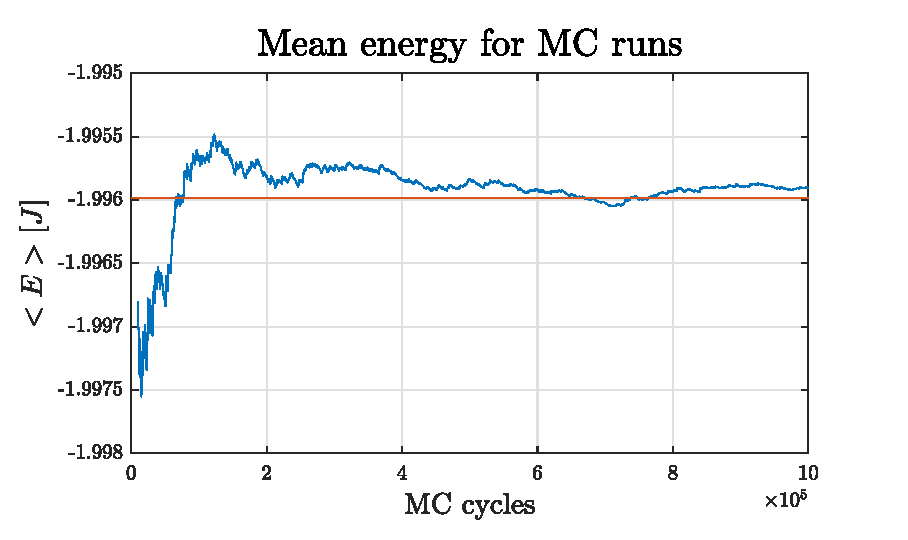
\includegraphics[width=0.5\textwidth]{2x2Energy}}
	\subfloat[]{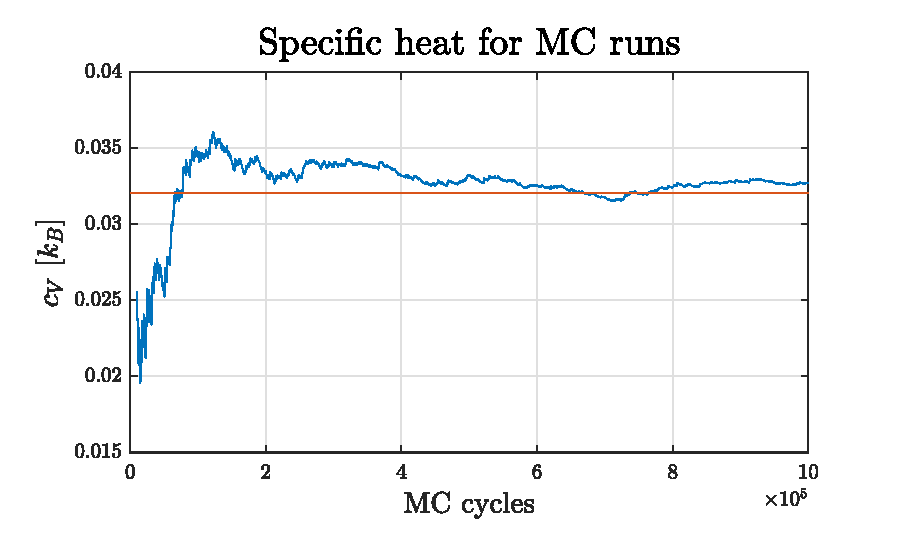
\includegraphics[width=0.5\textwidth]{2x2Cv}}\\
	\subfloat[]{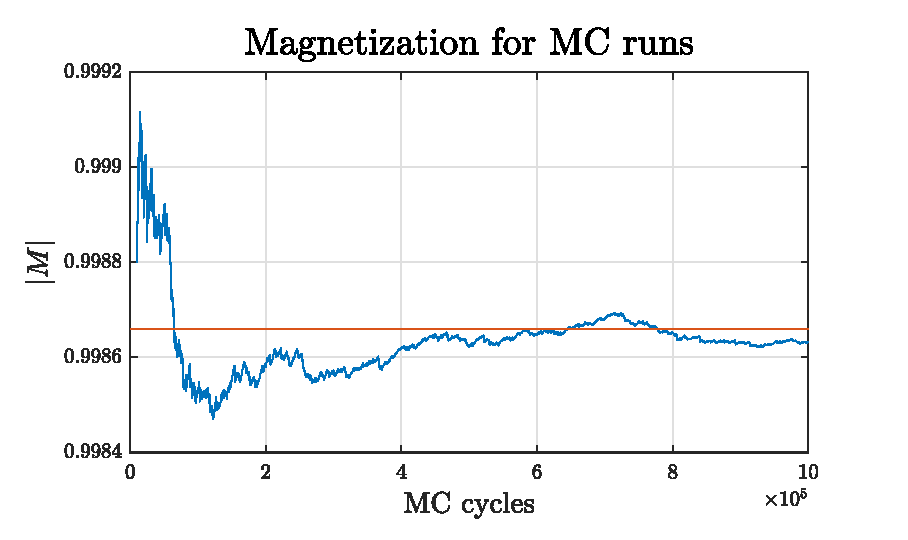
\includegraphics[width=0.5\textwidth]{2x2Magn}}
	\subfloat[]{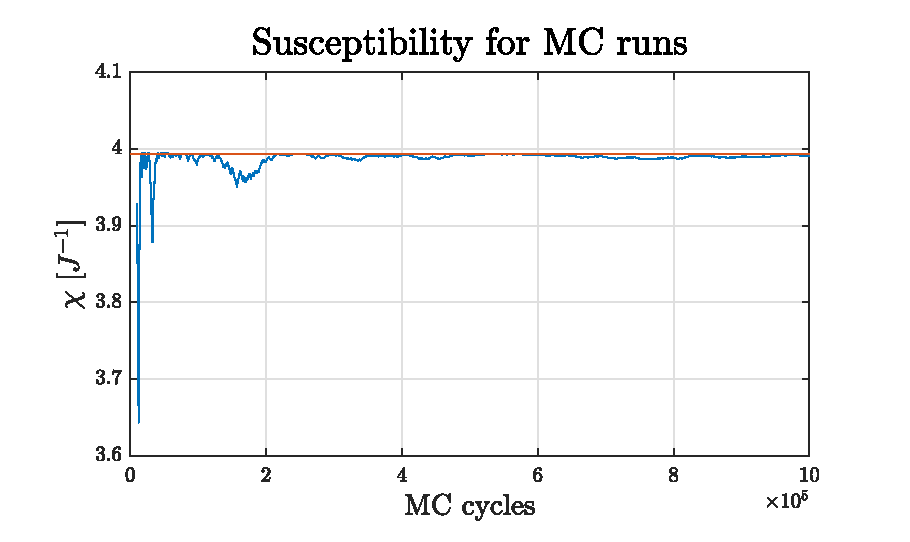
\includegraphics[width=0.5\textwidth]{2x2Chi}}
\caption{In the figure are shown the various expectation values computed after various MC runs. The theoretical values are also displayed as a straight red line.}
\end{figure*}
	
Therefore, to get good expectation values, we set the number of total MC cycles for the following simulations to be $10^6$.



\subsection{$20 \times 20$ lattice. Equilibrium state}
We increase the lattice size to $20\times20$ and keep the temperature $T=1.0\,Jk_B^{-1}$. The point is now to study the time needed to reach equilibrium, that is the number of monte Carlo cycles required for the fluctuations of the expectation values to be irrelevant. The results starting from an ordered lattice with all spins aligned up are shown in figure 2

\begin{figure*}[ht]
	\centering
	\label{20T1}
	\subfloat[]{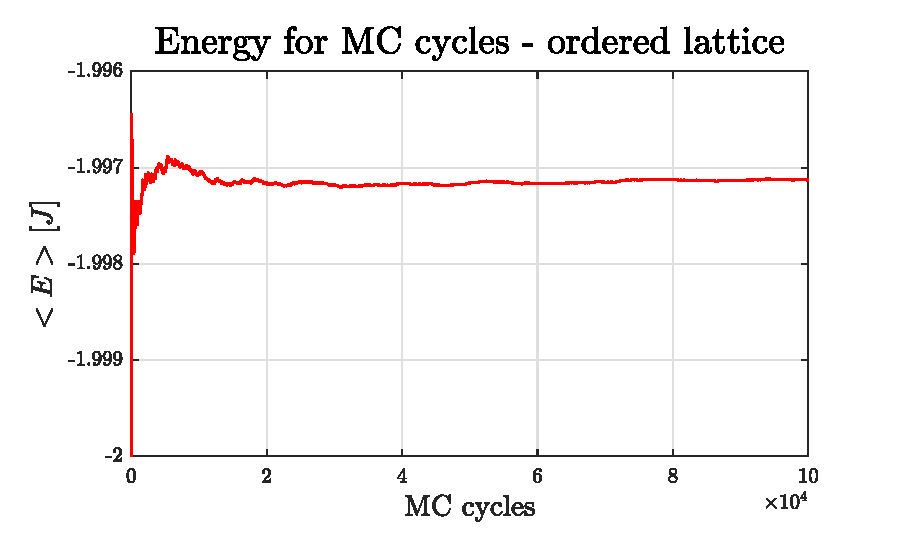
\includegraphics[width=0.4\textwidth]{20x20Energy}}
	\subfloat[]{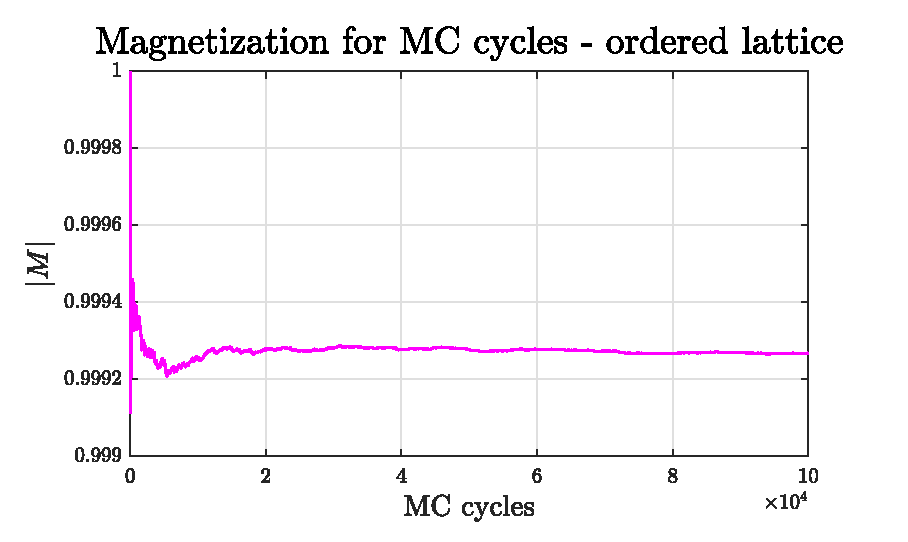
\includegraphics[width=0.4\textwidth]{20x20Magn}}
	\\
	\subfloat[]{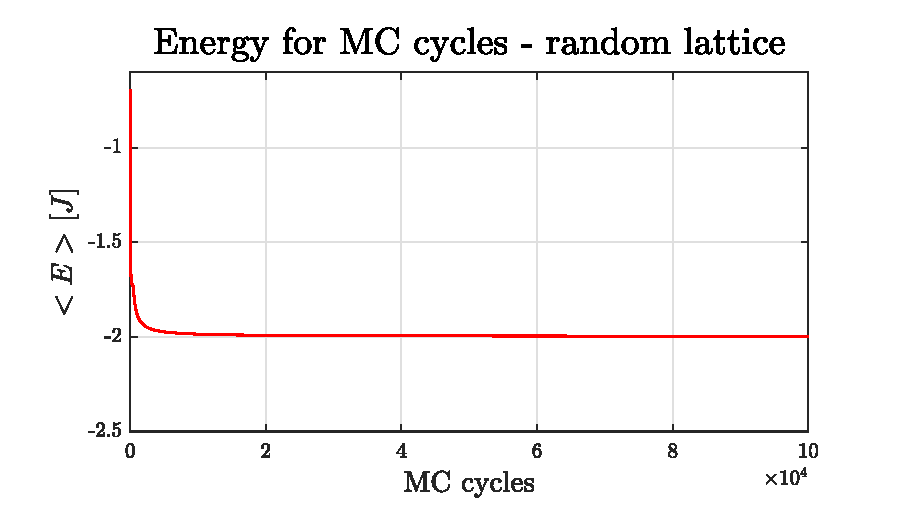
\includegraphics[width=0.4\textwidth]{20x20RandEnergy}}
	\subfloat[]{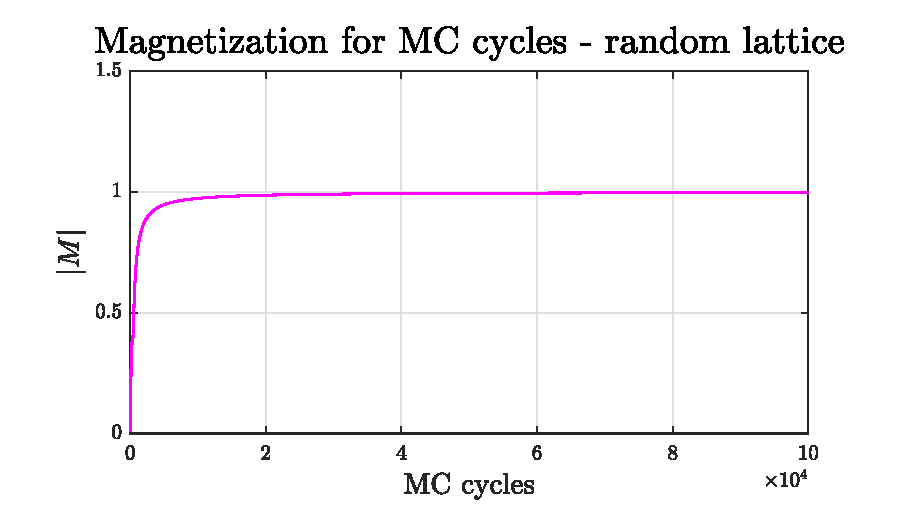
\includegraphics[width=0.4\textwidth]{20x20RandMagn}}
	\caption{The figure shows the evolution of the 20x20 system towards equilibrium at $T=1.0\,Jk_B^{-1}$ for the expectation values of respectively Energy and Magnetization in both the ordered case -(a) and (b)- and in the random case -(c) and (d)-.}
\end{figure*} 

If we do the same analysis starting from a random-spin lattice, we see that mean energy and magnetization at equilibrium converge to the same value. this means that for low temperatures, as we will discuss better later- the most likely state is an ordered one (we have a net magnetization) and there is a correlation between the spin domains in the lattice. The results for the random lattice are also shown in Figure 2.


We repeat the same analysis for a higher temperature $T=2.4\,Jk_B^{-1}$ (Figure 3). The equilibrium state has now different values for energy and magnetization. The temperature is high enough to drive the system towards a less ordinate state, where the net magnetization is lower than before end the mean energy is quite far from its minimum value. This is due to the fact that the potential for this system is Helmholtz' free energy, and the higher the temperature is, the more important the disorder of the system becomes for reaching the equilibrium state.

\begin{figure*}[ht]
	\label{20T2}
	\subfloat[]{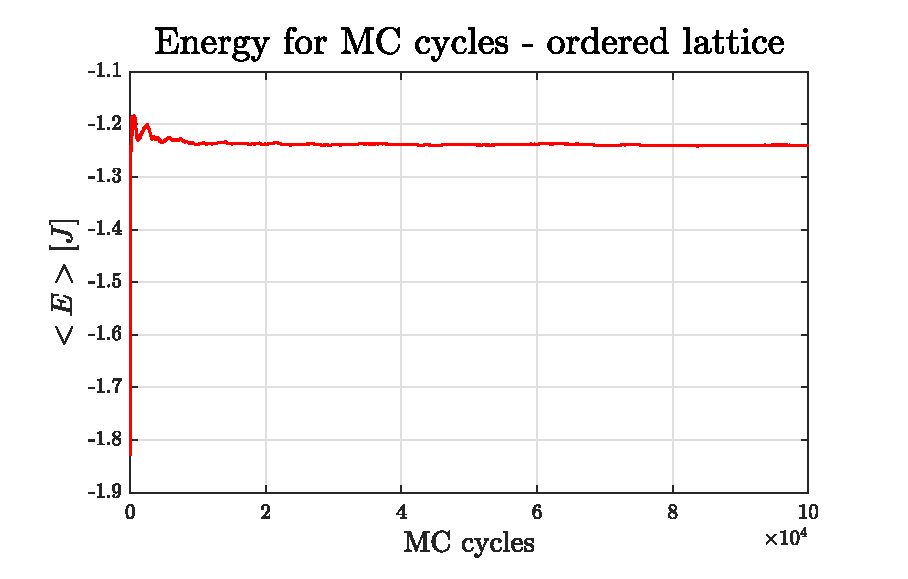
\includegraphics[width=0.4\textwidth]{20x20EnergyT2}}
	\subfloat[]{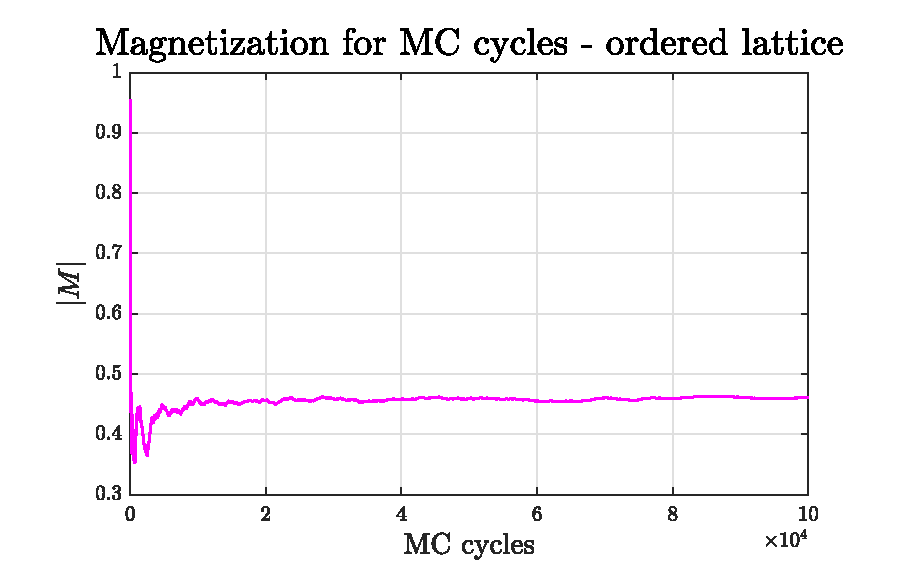
\includegraphics[width=0.4\textwidth]{20x20MagnT2}}
	\\
	\subfloat[]{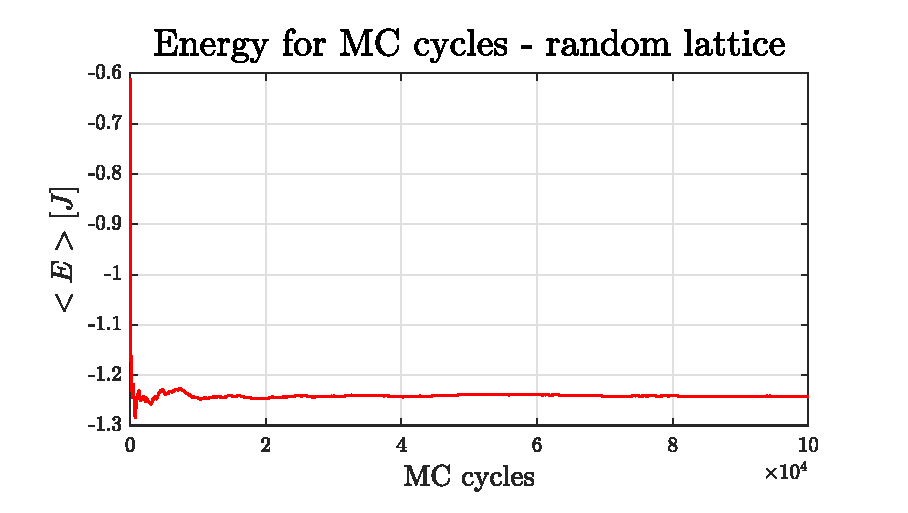
\includegraphics[width=0.4\textwidth]{20x20EnergyRandT2}}
	\subfloat[]{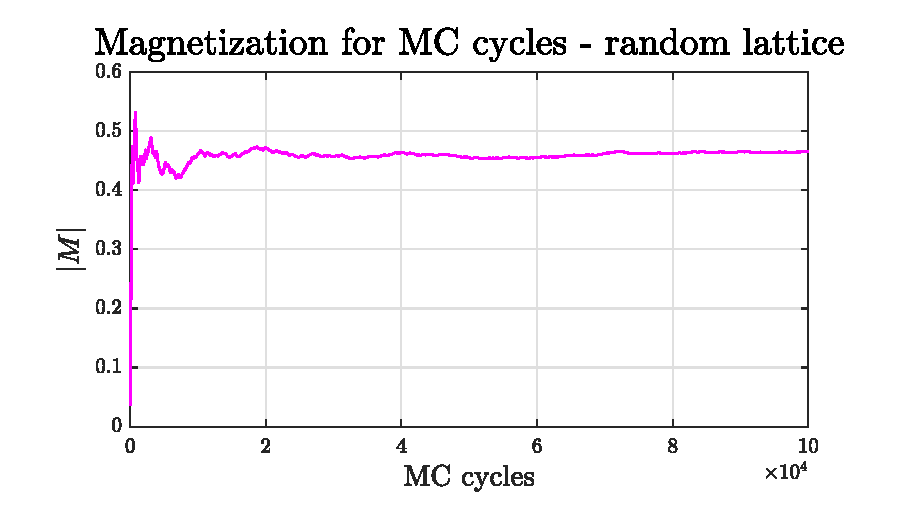
\includegraphics[width=0.4\textwidth]{20x20MagnRandT2}}
	\caption{The figure shows the evolution of the 20x20 system towards equilibrium at $T=2.4\,Jk_B^{-1}$ for the expectation values of respectively Energy and Magnetization in both the ordered case -(a) and (b)- and in the random case -(c) and (d)-.}
\end{figure*} 

Moreover, if we plot the accepted moves for MC cycle for both the values of temperature (Figure 4), we see that the trend is linear in both cases (there is the same probability to accept moves for every cycle) and does not depend on whether the initial lattice is random or ordered; the acceptance rate for the higher temperature is though much bigger. The reason for that is related to the Boltzmann distribution itself: the higher the temperature is, the wider the function becomes; this means that there are much more allowed states that the system can assume before reaching equilibrium. 

\begin{figure*}
	\label{AcceptedMoves}
	\subfloat[]{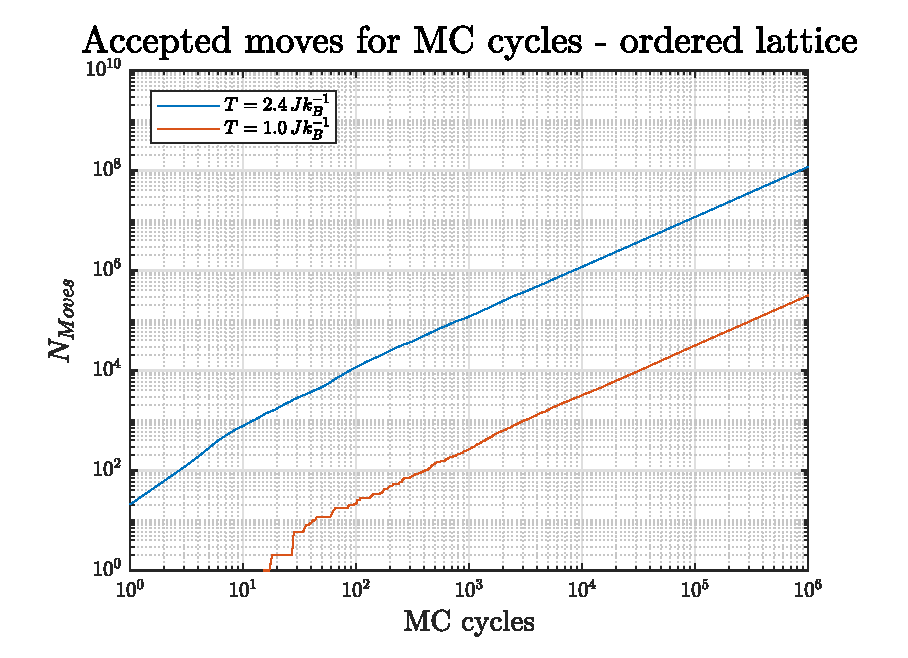
\includegraphics[width=0.4\textwidth]{AMOrdered}}
	\subfloat[]{\includegraphics[width=0.4\textwidth]{AMRandom}}
	\caption{The figure shows the number of accepted moves for the MC cycles performed in both ordered (a) and random (b) lattice.}	
\end{figure*}

Based on the plots for the various system we can estimate an equilibration time for the system that is about $2\times10^4$ MC cycles. For the next simulations, we will start the data sampling after equilibrium is reached, by introducing a cut off for the first $5\times10^4$ data.

\subsection{The Boltzmann distribution}
While running the simulations for the $20\times20$ lattice count now how often each value of energy appears in the system after the equilibrium state is reached, and get the distribution of energies after performing $9.5\times10^5$ MC cycles. 
The plots are shown in figure 5, where the counts have been normalized by the total number of cycles to get probabilities. Note that the x-axis value refers to the energy per spin.

\begin{figure*}[h!]
	\label{probabilities}
	\centering
	\subfloat[]{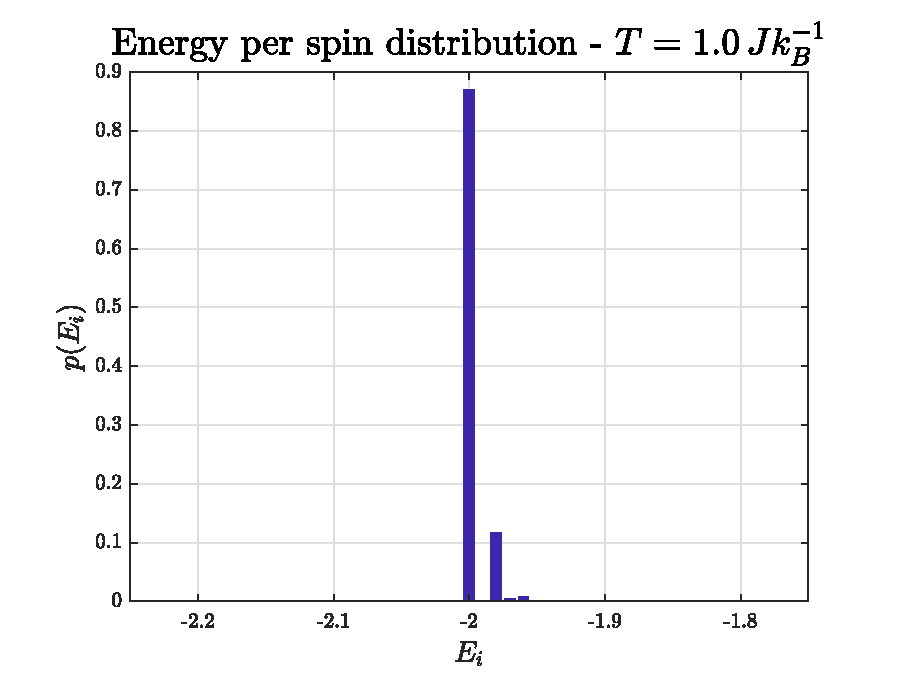
\includegraphics[width=0.4\textwidth]{ProbsT1}}
	\qquad
	\subfloat[]{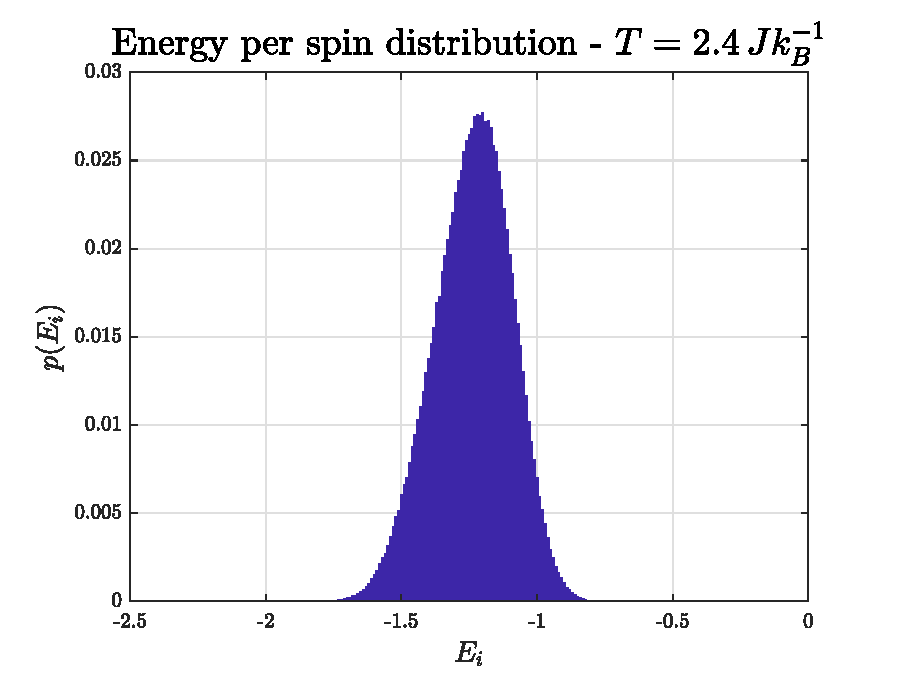
\includegraphics[width=0.4\textwidth]{ProbT2}}
	\caption{The figure displays the energy-per-spin distribution for the $20\times20$ lattice for $T=1.0\,Jk_B^{-1}$(a) and $T=2.4\,Jk_B^{-1}$(b). The data displayed refer to the random lattice, but for the ordered one the plots are the same since they both follow Boltzmann distribution.}
\end{figure*}

We clearly see that for the lowest temperature the accessible states are very few and condensed in a small interval; the lowest energy state $E=-2$ is the dominant one, with a probability of almost $\SI{90}{\percent}$, and the other states influence very little the mean value $\mean{E}=-1.997$. For the highest temperature, the energy distribution is more widespread since there are more accessible states and the peak of the distribution is on the mean value $E = -1.238$ (of course, both mean values of the distributions are the same values reached by the system at equilibrium -see Figures \ref{20T1Rand} and \ref{20T2Rand}-). We can see this also by considering the variances computed for both energies: $\sigma^2(T=1.0)=0.037$, $\sigma^2(T=2.4)=8.154$. Since the variance gives information of how much the data are spread with respect to the mean value, it is normal to expect a wider distribution for higher temperatures.

\subsection{Phase transitions and critical temperature}
Furthermore we run our code and generate data for different values of T from $2.1\,Jk_B^{-1}$ to $2.5\,Jk_B^{-1}$ for more MC cycles ($8\times10^6$) to see the behaviour of our expectation values close to the critical temperature $T_c$ (Figure 6). We can see different peaks in specific heat and susceptibility that indicate a second-order phase transition (ideally the values should diverge in the peak, but we do not have enough resolution), while mean Energy and Magnetization are continuous and present inflexion point in the correspondent peak. This makes sense since Mean energy and specific heat are respectively related to the first and second order temperature-derivative of Helmholtz free energy (since they are also related to the first and second order momentum of energy distribution, a similar argument can be used also for magnetization and susceptibility). Note tht to compute the susceptibility we use the mean absolute magnetization $|M|$, in order to have less fluctuations for a smaller lattice dimension.
\begin{figure*}
		\label{TransEV}
		\subfloat[]{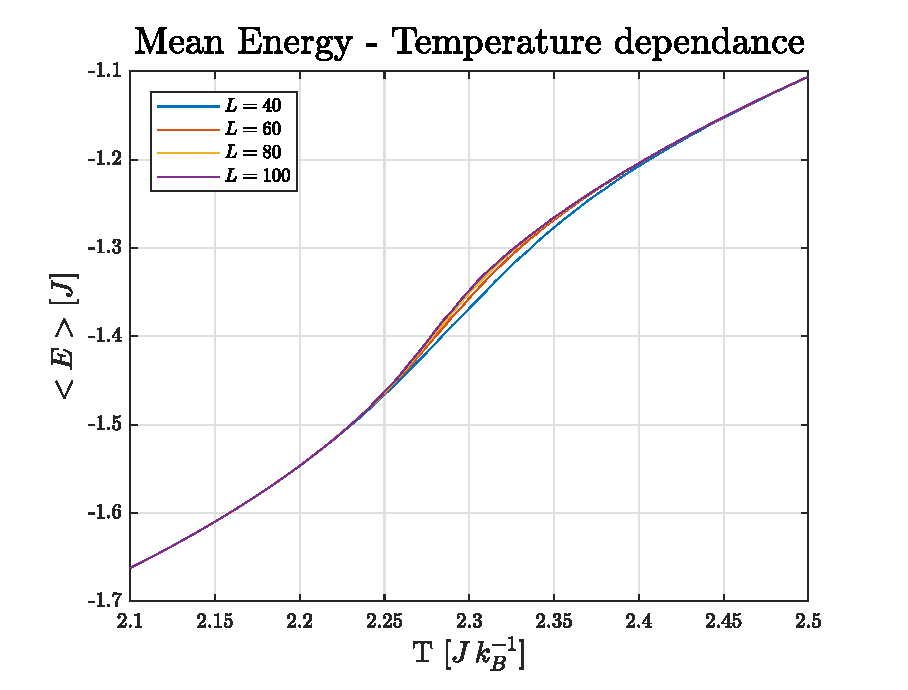
\includegraphics[width=0.4\textwidth]{TrangeEnergy}}
		\subfloat[]{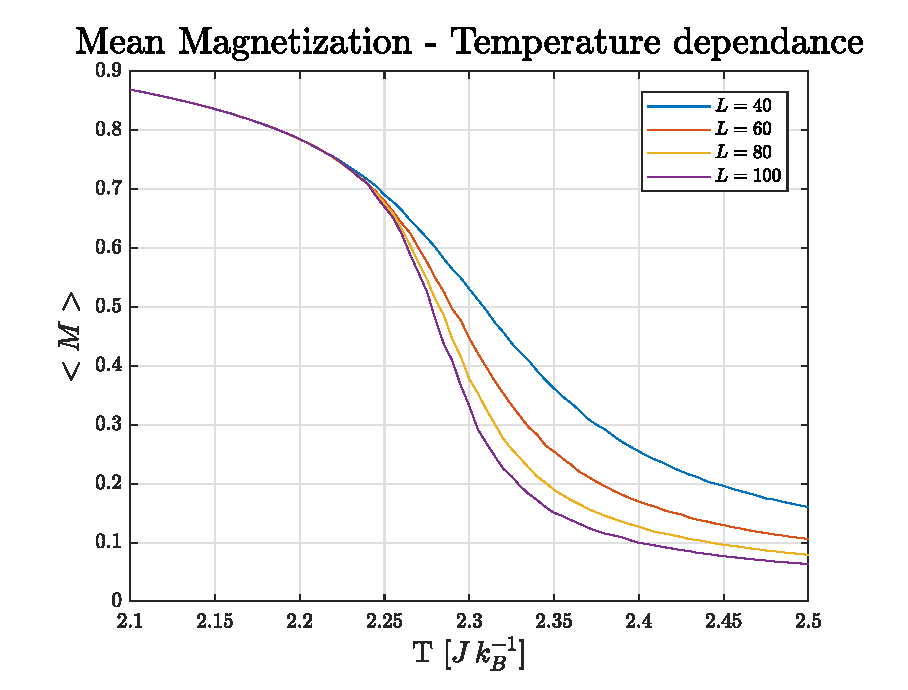
\includegraphics[width=0.4\textwidth]{TrangeM}}
		\\
		\subfloat[]{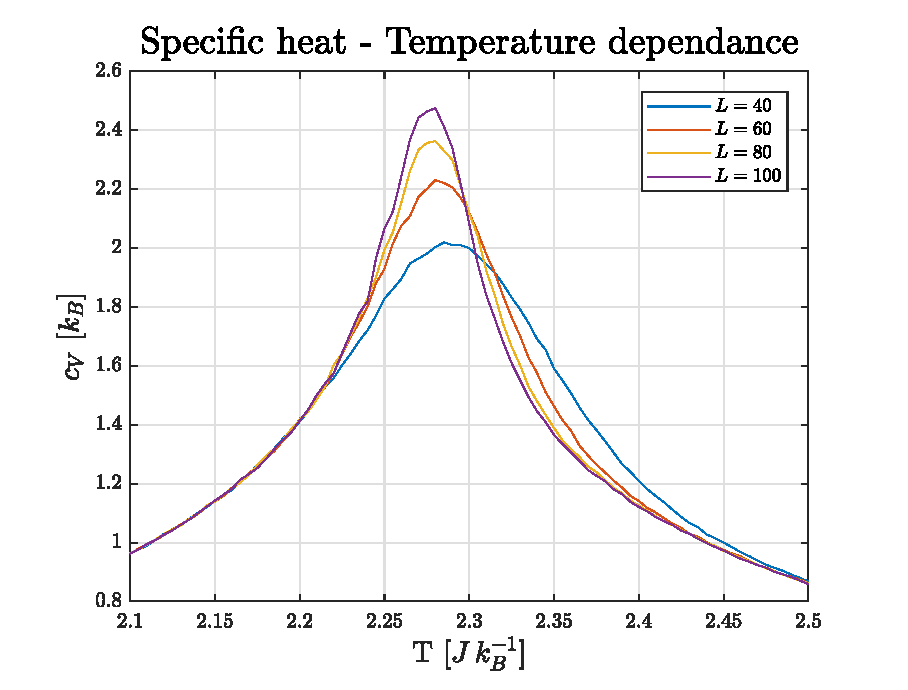
\includegraphics[width=0.4\textwidth]{TrangeCv}}
		\subfloat[]{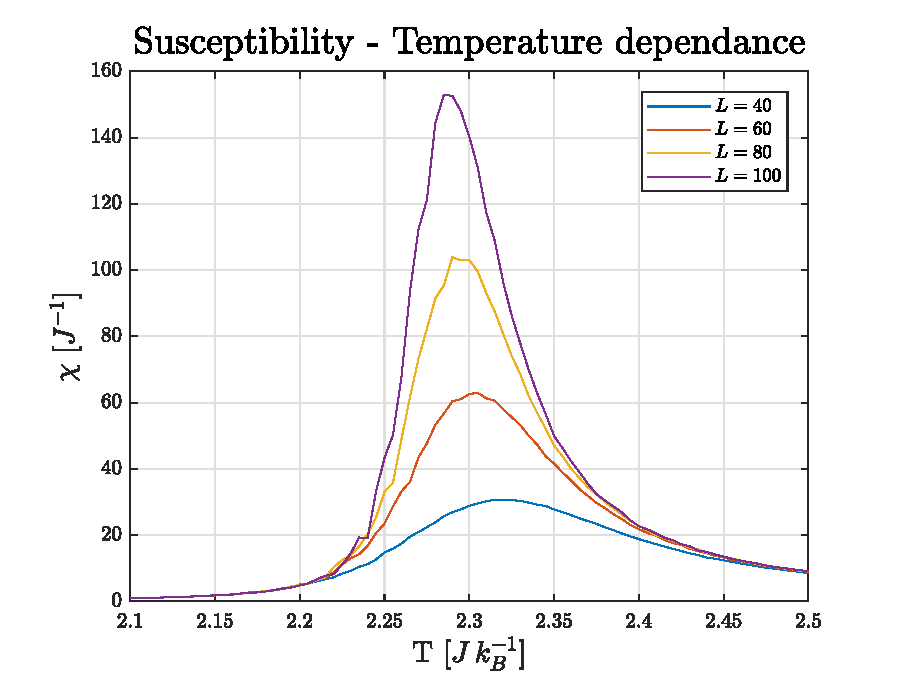
\includegraphics[width=0.4\textwidth]{TrangeChi}}
		\caption{The figure shows the behaviour of Energy, Magnetization, specific heat and susceptibility -(a), (b), (c), (d) respectively- for temperatures close to $T_c$ and for different lattice sizes.}
\end{figure*}

To find the critical temperature at $L=\infty$ we find the peaks of the susceptibility and then perform a linear fit (Figure 7) (with a standard data analysis function based on least squares method) on $L^{-1}$ to eq. \ref{critictemp}, with the result:
\begin{align*}
	T_c(L=\infty) = (2.261\pm0.008)Jk_B^{-1}
\end{align*}
The value is compatible with the exact one.

\begin{figure}[ht!]
	\centering
	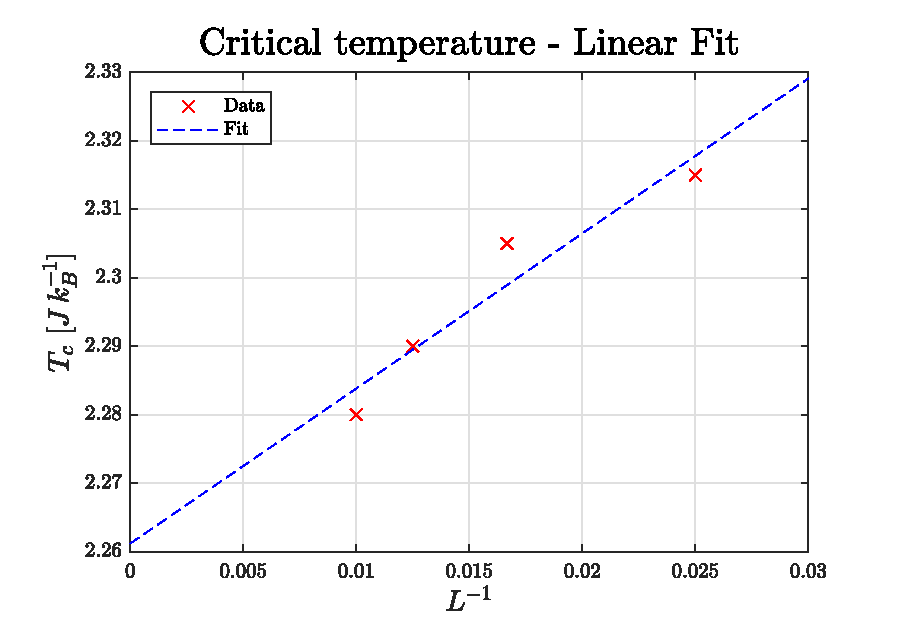
\includegraphics[width=0.47\textwidth]{TempFit}
	\label{LinFit}
	\caption{The figure shows the result of the linear fit on $L^{-1}$ to get the critical temperature for an infinite 2D lattice. The y-axis intercept is the value $T_c(L=\infty)$.}
\end{figure}

\section{Conclusions}
We analyzed a 2D binary thermodynamical system with Ising model for magnetization, in order to study its behaviour towards equilibrium and its phase transitions around a critical temperature.
At first we set a simple $2\times2$ system and see that to have a good compatibility between numerical and theoretical expectation vaues we need at least $5\times10^5$ Monte Carlo cycles. 
Then we increased the lattice dimension to $20\times20$ to see the evolution of the system towards the equilibrium status, reached after about $2\times10^4$ cycles. For this lattice we also studied the energy distribution of the states and saw that it obeys the Boltzmann distribution.
Eventually we ran our code for bigger lattices (40, 60, 80, 100) and analyzed the behaviour of the expectation values when the temperature changes. We managed to characterize the second-order phase transition for our magnetic system and, by detecting the critical temperatures of the susceptibility for different temperatures and performing a linear fit, we managed to extend our results to an infinite 2D lattice, which has a critical temperature of $(2.261\pm0.008)Jk_B^{-1}$. This value is compatible with the exact one by L. Onsager.
These simulations are an example of how efficient Metropolis algorithm is to simulate complex systems without a deep theoretical and analytical background. This characteristic allows this method to be applied in an enormous amount of situation (for example, the evolution of any macroscopic system under certain conditions).
I would eventually like to acknowledge the precious help and patience of Davide Saccardo, and thank him for the interesting discussions and the fundamental support with some "hardware" problems.

\begin{thebibliography}{5}

\bibitem[1]{compnotes} M. H. Jensen, \textit{Computational physics - Lecture notes Fall 2015}, University of Oslo - Department of Physics, 2015. 
\end{thebibliography}

\end{document}
%
% ****** End of file apssamp.tex ******